\section{Реализация алгоритма}\label{ps}

Прежде чем приступать к реализации модификации приведем пример, иллюстрирующий мотивацию предлагаемой модификации.

\subsection{Мотивация}

В классическом GLL алгоритме дескриптор содержит в себе \emph{позицию в грамматике} --- текущую обрабатываемую продукцию и позицию в этой продукции, обозначающаю какие элементы продукции уже были обработаны.
Таким образом для каждой продукции грамматики в GLL алгоритме неизбежно создается как минимум столько дескрипторов, сколько в этой продукции символов.

\begin{ruexample}
    Рассмотрим простой язык, состоящий из нуля и более повторений буквы $a$: $\mathbb{L}_1 = \{a\}^*$.
\end{ruexample}

\begin{ruexample}
    Контекстно-свободная грамматика $\mathbb{G}_1$, задающая язык $\mathbb{L}_1$.
    $$S \longrightarrow a S$$
    $$S \longrightarrow \varepsilon$$
\end{ruexample}
Для такой грамматики в ходе работы GLL алгоритма будет создано целых четыре \emph{позиции в грамматике}, и, соответственно, не меньше четырех дескрипторов.

Однако этот же язык можно выразить с помощью рекурсивного автомата всего на одном состоянии и одном переходе, а для такого автомата количество созданных GLL алгоритмом дескрипторов будет гораздо меньше.

\begin{ruexample}
    Рекурсивный автомат $\mathbb{A}_1$, задающий язык $\mathbb{L}_1$.

    \begin{align}
    \label{input2}
        \begin{tikzpicture}[node distance=2.5cm,shorten >=1pt,on grid,auto]
           \node[state, initial, accepting] (q_0)   {$0 \{S\}$};
            \path[->]
            (q_0) edge[loop, above]  node {a} (q_0);
        \end{tikzpicture}
    \end{align}

\end{ruexample}

Так как производительность GLL алгоритма напрямую зависит от количества создаваемых дескрипторов, возникает предположение о модификации классического GLL алгоритма путем замены контекстно-свободной грамматики на рекурсивный автомат.

\subsection{Особенности реализации} 

Предлагаемая в данной работе модификация GLL алгоритма основана на замене в дескрипторе \emph{позиции в грамматике} на состояние рекурсивного автомата, то есть в четверке $\langle \langle A \rightarrow \alpha, c_{\alpha} \rangle, c_{u}, c_{i}, c_{N} \rangle$ пара $\langle A \rightarrow \alpha, c_{\alpha} \rangle$ заменяется на $c_{R}$ --- текущее состояние рекурсивного автомата.
Соответственно переход в контекстно-свободной грамматике заменяется на переход в рекурсивном автомате.

Данная модификация, как и классический GLL алгоритм, может быть обобщена на графы --- на шаге перехода в рекурсивном автомате обрабатываются все переходы из текущего состояния рекурсивного автомата по всем исходящим ребрам текущей вершины графа.

Одной из недавних удачных реализаций GLL алгоритма является библиотека GLL4Graph\footnote{Github репозиторий библиотеки: \url{https://github.com/FormalLanguageConstrainedPathQuerying/GLL4Graph}. Accessed: 05/04/2023}, написанная на языке программирования Java.
Это означает, что виртуальная машина Java, она же JVM, является подходящей для эффективной реализации такого рода алгоритмов.
С другой стороны, опираясь на то, что данная работа является возможной основой для дальнейших расширений и оптимизаций, не менее важным было не только разработать оптимальную для этих целей архитектуру, но и сделать сам код реализации максимально лаконичным и понятным.
По сравнению с языком программирования Java, программа, написанная на языке программирования Kotlin имеет более читаемый и структурно точный код, что облегчает не только ее понимание, но и дальнейшую поддержку. 
Поэтому в качестве языка программирования для реализации модификации GLL алгоритма был выбран язык Kotlin.

\subsection{Архитектура}

Прежде, чем приступать к модификации GLL алгоритма, необходимо реализовать его классический вариант.
В связи с этим возникает вопрос о разработке подходящей архитектуры для проекта в целом.
Поэтому были разработаны следующие требования.
\begin{itemize}
    \item Для удобства модификации и дальнейшей поддержки кода каждая реализация GLL алгоритма должна находиться в отдельном модуле и не зависеть от других реализаций.
    \item Кроме GLL алгоритмов, с входными данными, представленными в виде строки, необходимо реализовать GLL алгоритмы, с входными данными, представленными в виде графа.
    \item Помимо решения задачи поиска путей в графе с контекстно-сво-бодными ограничениями необходимо поддержать решение задачи поиска достижимостей в графе с контекстно-свободными ограничениями.
    \item Наконец, необходимо предоставить некоторый удобный пользователю интерфейс с возможностью выбора конкретного сценария для GLL алгоритма.
\end{itemize}
Для удовлетворения поставленным требованиям была разработана следующая архитектура.

\begin{figure}[H]
    \centering
    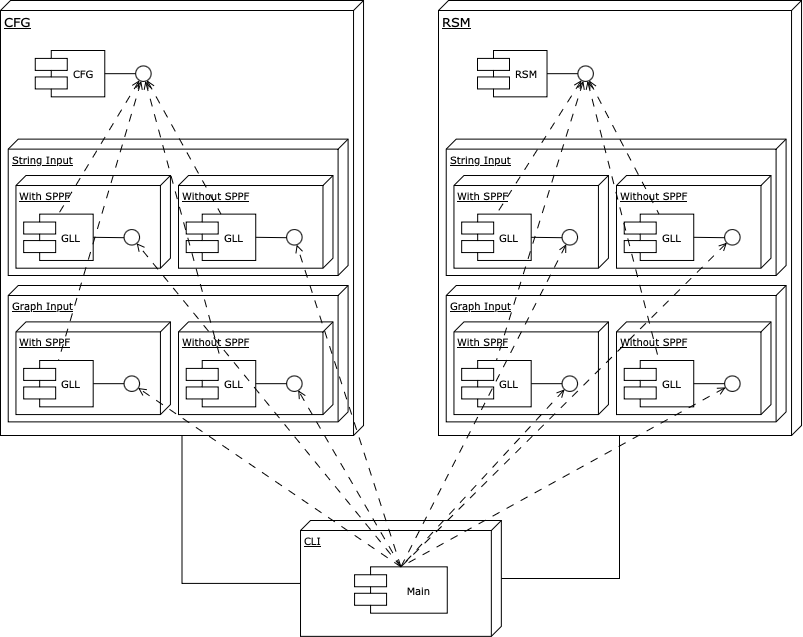
\includegraphics[width=\textwidth]{matmex-diploma-template-master/figures/architecture.png}
    \caption{Архитектура проекта}
    \label{fig:architecture}
\end{figure}

Разработанный проект имеет блочно-модульную архитектуру.
Диаграмма включает в себя три основных блока --- снизу блок, содеражащий модуль, реализующий интерфейс командой строки, который был отделен от модулей реализаций GLL, сверху слева блок, представляющий собой реализации GLL алгоритма на основе контекстно-свободных грамматик, имеющий общий модуль представления контекстно-свободной грамматики для всех GLL алгоритмов в блоке, сверху справа --- блок, представляющий собой реализации GLL алгоритма на основе рекурсивного автомата, имеющий общий модуль представления рекурсивного автомата для всех GLL алгоритмов в блоке.
Для обоих типов реализации были инкапсулированы в отдельные блоки сценарии выполнения алгоритма для входных данных в виде строки и для входных данных в виде графа.
Внутри последних в свою очередь были инкапсулированы сценарии с построением дерева разбора SPPF и без построения дерева разбора.

Данная архитектура позволяет не только максимально гибко задавать параметры для запуска алгоритма через интерфейс командой строки, но и облегчает понимание и поддержку кода, так как реализаци GLL алгоритмов имеют строгую иерархию и независимы между собой. 